\documentclass[stochastic-or.tex]{subfiles}
\usepackage{amsmath} % this is only used to enforce good environment completion in emacs
\externaldocument{stochastic-or}

\loadgeometry{tufte}

\begin{document}

\section{Applications of Level-crossing, Little's law and PASTA}
\label{sec:mnmn1}

In this section we apply the tools developed above to a number of interesting queueing systems.
Specifically, we discuss in detail how to plan the number of cashiers at a supermarket such that the average queue length remains small.
Note that in many queueing systems, the manager should balance the cost of the waiting time of customers against the cost of idle servers; recall in queueing systems always somebody has to wait, either a customer in queue or a server being idle.





\newthought{Let us next} discuss the example of cashier planning at a supermarket.
Here we keep the models simple, but we include all necessary steps to solve the a realistic planning problem.
Note that many service systems, e.g.
hospitals, deal with similar personnel planning problems to cover stochastic demand.


We start with specifying the \emph{arrival process}.
It is reasonable to model it as a Poisson process, as there are many potential customers, each choosing with a small probability to go to the supermarket at a certain moment in time.
Thus, we only have to characterize the arrival rate.
Estimating this for a supermarket is easy because the cash registers track all customers payments.  This provides us with the departure time of each customer, hence we can use this to estimate the average number of arrivals per hour.

It is common to use a \emph{demand profile} which shows the average number of customers arriving per hour.
\begin{marginfigure}
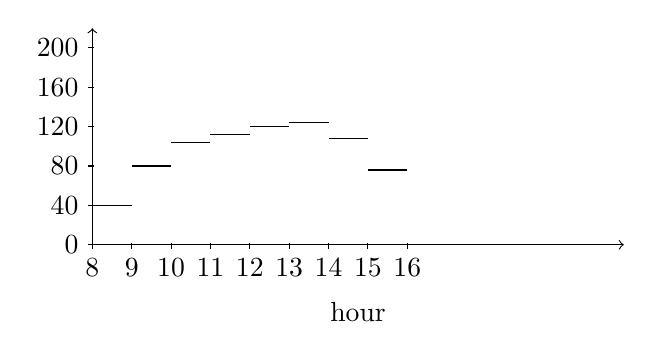
\begin{tikzpicture}[scale=.5]
    %axis
    \draw[->] (0,0) -- coordinate (x axis mid) (13.5,0);
    \draw[->] (0,0) -- coordinate (y axis mid) (0,5.5);
    %ticks
    \foreach \x in {0,...,8}
 \pgfmathsetmacro{\my}{int(\x+8)}
        \draw (\x,1pt) -- (\x,-3pt)
            node[anchor=north] {$\my$};
    \foreach \y in {0,...,5}
 \pgfmathsetmacro{\my}{int(\y*40)}
        \draw (1pt,\y) -- (-3pt,\y)
            node[anchor=east] {\my};
%labels
\node[below=0.6cm] at (x axis mid) {hour};
%\node[rotate=90, left=1.2cm] at (y axis mid) {$\lambda$};

\draw (0,1)--(1,1);
\draw (1,2)--(2,2);
\draw (2,2.6)--(3,2.6);
\draw (3,2.8)--(4,2.8);
\draw (4,3.)--(5,3.);
\draw (5,3.1)--(6,3.1);
\draw (6,2.7)--(7,2.7);
\draw (7,1.9)--(8,1.9);
% \draw (8,2.5)--(9,2.5);
% \draw (9,3.3)--(10,3.3);
% \draw (10,3.5)--(11,3.5);
%\draw (11,2.3)--(12,2.3);
%\draw (12,1.2)--(13,1.2);
\end{tikzpicture}
\caption{A demand profile.}
\label{fig:loadprofile}
\end{marginfigure}
Then we model the arrivals as a Poisson process with an arrival rate that is constant during a certain hour as specified by the demand profile.


It is also easy to find the\emph{ service distribution} from the cash registers.
The first item scanned after a payment determines the start of a service, and the payment closes the service. For ease, we model the service time distribution as exponential with mean $1.5$ minutes.

For the \emph{service objective} we prefer to keep the average number of people in the system such that $\E L \leq 5$. (Other KPIs are also possible to use.)

Let us model the situation as an $M/M/1$ queue with a fast server, so that it is easy to find the smallest number of servers necessary to prevent the queue from exploding.
Since $\E L = \rho/(1-\rho)$, and $\rho=\lambda \E S /c$, solving for~$c$ in the inequality $\E L \leq 5$ gives
\begin{equation*}
c \geq \frac 6 5 \lambda \E S \approx 0.03 \lambda,
\end{equation*}
where, with  the above estimate, $\E{S}=1.5/60$ hour.
It's easy to apply this formula. For instance,  we see in the demand profile~\cref{fig:loadprofile} that $\lambda= 120$ customers per hour between 12 and 13, hence $c\approx 3.8 = 4$.

With this we can find a formula to convert the demand profile into a \emph{load profile} to specify the minimal number of servers per hour needed to meet the service objective.


\newthought{The last step} in the planning process is to \emph{cover the load profile with service shifts}.
This is typically not easy since shifts have to satisfy all kinds of restrictions with respect to breaks and durations.  Moreover, shifts can also have different costs: evening shifts are typically  more expensive per hour.

The usual way to solve such covering problems is by means of an integer
problem. For instance, suppose only 4 \emph{shift plans} are available as shown at the right.\sidenote{\begin{enumerate}
\item $++-++$
\item $+++-+$
\item $++-+++$
\item $+++-++$,
\end{enumerate}
Shift plans. A $+$ indicates a working hour and $-$ a break of an hour.}

For the optimization, let $x_i$ be the number of shifts of type~$i$ and~$c_i$ the cost of this type.
Then the problem is to solve $\min \sum_i c_i x_i$,
such that for all hours~$t$ the shifts cover the load, i.e., $\sum_i x_i \1{t \in s_i} \geq 0.03 \lambda_t$.
(We write $t\in s_i$ if hour~$t$ is covered by shift type~$i$.)

\newthought{Finally, we need} to address the quality of our approximation: to simplify we used the $M/M/1$ queue with a fast server, while we know that in a supermarket there are often multiple parallel cashiers. Specifically, we are interested in the ratio $\E{\L(M/M/c}$ and $\E{L(M/M/1)}$ where in the $M/M/1$ queue the server works at rate~$c$.

To understand this better, we consider a numerical example.
Suppose that we have an $M/M/3$ queue with $\lambda = 5$ per day and $\mu=2$ per day per server, and we compare $\E L$ of this queue to that of an $M/M/1$ queue with the same arrival rate but with a service rate of $\mu = 3\cdot 2 = 6$.
\begin{marginfigure}
\includegraphics{../figures/mm3_vs_mm1.pdf}
\caption{The ratio of $\E\L$ for the $M/M/3$ and $M/M/1$ queue.}
\label{fig:fast}
\end{marginfigure}

\cref{fig:fast} shows  the ratio of $\E\L$ for both queues as a function of $\rho$.
Clearly, when $\rho$ is small, this ratio is about~$3$.
This is reasonable, because the service time in the fast $M/M/1$ is 3 times as small as the service time in the $M/M/3$ queue.  Thus, when $\rho$ is small, the time in queue is small, hence $\E\J \approx \E S$.
However, when $\rho$ is large, $\E\J \gg \E S$, so that in this case, the ratio between the queue lengths becomes approximately 1.

In our supermarket model, $\rho=5/6$, hence the approximation is not too bad.

Here is the code I used to make~\cref{fig:fast}.
\begin{python}
from math import factorial
import numpy as np
import matplotlib.pylab as plt

from latex_figures import fig_in_latex_format


def EL(labda, mu, c):
    rho = labda / mu / c
    G = sum((c * rho) ** n / factorial(n) for n in range(c))
    G += (c * rho) ** c / ((1 - rho) * factorial(c))
    Q = (c * rho) ** c / (factorial(c) * G) * rho / (1 - rho) ** 2
    L = Q + labda / mu
    return L


mu, c = 2.0, 3

L, load = [], []

for labda in np.linspace(0.1, 5.8, 20):
    L.append(EL(labda, mu, c) / EL(labda, c * mu, 1))
    load.append(labda / mu / c)


def cm_to_inch(cm):
    return cm / 2.54


plt.figure(figsize=(cm_to_inch(5), cm_to_inch(6)))
plt.plot(load, L, label=r"$L_3/L_1$", lw=0.7)
plt.xlabel("$\\rho$")
plt.legend()
plt.tight_layout()
plt.savefig("../figures/mm3_vs_mm1.pdf")
\end{python}


\begin{truefalse}
    Suppose $\frac{\lambda}{\mu} = 2$ then we claim that 3 is the minimum number of servers required to make the system stable.
    \begin{solution}
        True.
    \end{solution}
\end{truefalse}

\begin{truefalse}
Claim: It is always better to have a single fast server than multiple slow servers which together have the same rate.
    \begin{solution}
    False.
This depends on the objective.
The service time at a slow server is longer.
However, when multiple servers are present, if one server breaks down, service can still continue with the other servers, while when a single fast server fails, everything stops.
    \end{solution}
\end{truefalse}

\begin{truefalse}
A repair/maintenance facility would like to determine how many employees should be working in its tool crib.
The service time is exponential, with mean 4 minutes, and customers arrive as a Poisson process with rate 28 per hour.
With one employee we claim that the system is not rate stable.
\begin{solution}
True.
\end{solution}
\end{truefalse}


\begin{truefalse}
Consider an $M/M/c/K$ queue that is not rate stable, but  jobs sometimes balk. Claim: $\lim\limits_{t\to\infty}\mathbb{P}(L(t)=K)=1$.
\begin{solution}
  False. Just after jobs balk, the number of jobs in the system is less than $K$.
\end{solution}
\end{truefalse}



\newthought{The next exercises require} quite some modeling skills. Hence, they may be quite hard even thought the formulas are simple.

\begin{exercise}
In the town hall of the municipality, people can, for example, renew their driver's license or passport.
For ease, assume there is just one employee, and that the arrivals of customers are not planned.
Why is it reasonable to model this queueing system as a $M/M/1$ queue?

Measurements show that $\E \W = 6$ minute, and $\lambda=5$ per minute.
What are the service rate and utilization?
Calculate $\E{\QQ}$, $\E \L$.

There should be a sufficient number of seatings so that all waiting customers can sit down at least 90 percent of the time.
How many seatings should there minimally be? What would you advice to the municipality?
\begin{hint}
  $\E{\QQ}$ follows right away from an application of Little's law.
  For the other quantities we need to find $\E S$.
  Use the expression for  $\E\W$ for the $M/M/1$ queue to solve for $\rho$. Then, since $\lambda$ is known, $\E S$ follows.
\end{hint}
\begin{solution}
As people arrive without making appointments, it is reasonable to say that the inter-arrival times are memoryless.
As for the services, the employee deals with many different questions, some are short, some are long.
So, we model service times as exponential too.

With Little's law:
\begin{pyconsole}[municipality]
labda = 5. # per minute
EW = 6.
EQ = labda * EW
EQ
\end{pyconsole}

We can use the expression for $\E\W$ to solve for $\rho$, but we can also do a simple search.
\begin{pyconsole}[municipality]
from scipy.optimize import bisect

EW = 6.

def find_W(rho):
    # return W -1 for given rho
    ES = rho / labda
    return rho / (1 - rho) * ES - EW


rho = bisect(find_W, 0, 0.999)
rho
ES = rho / labda
ES
J = EW + ES
J
L = labda*J
L
\end{pyconsole}
Next, find~$n$ such that $\sum_{j=1}^n p_j > 0.9$.
We start counting at 1, because while the system contains one job, this customer is in service, hence stands at desk of the employee.
\begin{pyconsole}[municipality]
n, p = 0, 1 - rho
total = p
while total <= 0.9:
    p *= rho
    total += p
    n += 1

total
n - 1
\end{pyconsole}
Note that the while loop breaks when~$n$ is one too large.

The average queue is huge: hire an extra employee.
\end{solution}
\end{exercise}




\begin{exercise} The smallest barber shop in town works alone and has two chairs for waiting customers.
 Six jobs arrive per hour, and the barber needs 12 minutes for a hair cut. We model this, for ease, as an $M/M/1/3$ queue.
 Estimate $\E{\QQ}$ and the average number of customers served per hour.
 Then, estimate $\E{\QQ}$ when the barber hires another location that allows for 3 extra chairs.
 Quantify the effect on the number of customers served per hour.
\begin{solution}
This is an $M/M/1/3$ queue: there is room for 1 customer in service and two in queue.

We import \mintinline{python}{numpy} and convert the lists to arrays is to fix the output precision to 3, otherwise we get long floats in the output.

First the case with $b=2$.
\begin{pyconsole}[barber]
import numpy as np
np.set_printoptions(precision=3)

labda, mu, c = 6.0,  5.0, 1
rho = labda / mu
K = c + 2


p = np.array([rho ** n for n in range(K + 1)]) # range(n) is up to n
G = sum(p)
p /= G  # normalize
p
L = sum(n * p[n] for n in range(len(p)))
L
Q = sum(max(n - c,0) * p[n] for n in range(len(p)))
Q
lost = labda * p[-1]  # the last element of p
labda - lost # accepted, hence served
\end{pyconsole}

Now with three extra chairs.

\begin{pyconsole}[barber]
K += 3
K
p = np.array([rho ** n for n in range(K + 1)]) # range(n) is up to n
G = sum(p)
p /= G  # normalize
lost = labda * p[-1]  # the last element of P
labda - lost # accepted, hence served
\end{pyconsole}
We see that since the server is overloaded, the acceptance is not much affected by increasing the number of chairs.
We need an extra server.
\end{solution}
\end{exercise}



\begin{exercise}\label{ex:39}
Occasionally there is pizza stand at the corner of the Verlengde Visserstraat and the Westersingel in Groningen.
As people (tend to) behave like sheep, the rate at which people join the queue depends on the actual queue length. When there is nobody waiting, people are somewhat hesitant to order: `When there are no people waiting, most probably the pizzas are not good.'. However, when the queue is long, people prefer to go elsewhere.
Measurements show that the number of arrivals per hour is well captured by the array
\mintinline{python}{labda = np.array([10.0, 10.0, 20.0, 20.0, 5.0])}.
The pizza oven can contain two pizzas, and it takes 2 minutes to bake a pizza. We model the system as an $M/M/2$ queue.

Calculate the steady state probabilities, and from this  the average arrival rate. Then, find $\E \L$, $\E{\QQ}$, $\E \J$ and $\E{\W}$.
\begin{solution}
The computations.
\begin{pyconsole}[pizza]
import numpy as np
np.set_printoptions(precision=3)

labda = np.array([10.0, 10.0, 20.0, 20.0, 5.0])
mu = np.array([0., 30., 60., 60., 60., 60.])
c = 2

p = np.ones_like(mu)
for i in range(len(labda)):
    p[i+1] = labda[i] *p[i]/ mu[i+1]

p /= p.sum()
p
labdaBar = sum(labda[n] * p[n] for n in range(len(labda)))
labdaBar
L = sum(n * p[n] for n in range(len(p)))
L
Q = sum(max(n - c,0) * p[n] for n in range(len(p)))
Q
J = L / labdaBar
J
W = Q / labdaBar
W
\end{pyconsole}

\end{solution}
\end{exercise}




\begin{exercise}\label{ex:95}
Fast food restaurants tend to fry pattys before customers arrive.
Like this they can serve customers faster, because when a customer arrives while there is still an inventory of prepared pattys, the server only has to flip a patty in a bun, while otherwise the customer has to wait for the additional frying time of the patty.
Assume the restaurant keeps at most 3 pattys on stock.
To keep the model simple, assume the restaurant has just one pan to fry a patty and the frying time $S\sim \Exp{\mu}$ with $\mu = 15$ per hour.
Customers arrive as a Poisson process with rate $\lambda=12$ per hour.
When there is prepared patty upon arrival, the customer is served immediately, otherwise the customer has to wait for a patty.

Explain how to model this system as an $M/M/1$ system.  Then compute the average number of pattys on stock, the average number of people waiting, and the average waiting time of a patty before it ends up in a bun, and the average time a person has to wait for a hamburger.

You should remember this problem.
It is of fundamental importance in inventory control and known as an \emph{inventory system with backlogging}; it is (implicitly) used by nearly any company that keeps inventory.
\begin{hint}
Let~$T$ be the number of pattys waiting and~$G$ the number of persons waiting.
There cannot be a patty and a person waiting at the same time, hence $T\cdot G = 0$.
Take~$L$ as the number of jobs in an $M/M/1$ queue.
If $L=0$, then there are 3 pattys on stock, when $L=1$ there is one patty less $T=2, G=0$; when $L=2$, we have two pattys less, so $T=1, G=0$, when $L=3$, there are no pattys on stock, but also no people waiting, hence $T=0, G=0$.
When $L=4$, we ran out of pattys and one person must be waiting, hence $T=0, G=1$.

With this reasoning we see a pattern:  at all moments in time, $3=T+L - G$.
Now map this system to an $M/M/1$ queue.
\end{hint}
\begin{solution}
From the hint, the rv~$L$ behaves like the number of jobs in an $M/M/1$ queue. If we have~$L$, then with the two properties $T G = 0$ and $3 = T +L - G$, we can retrieve (uniquely at all moments in time) the number of pattys~$T$ on stock and the number of people waiting~$G$. In inventory terms, $G$ represents the number of \emph{backlogged} pattys.

With this mapping, the expected number of pattys on stock is $\E T =  \sum_{l=0}^3 (3-l)p(l)$.
\begin{pyconsole}[taxis]
labda = 12.0  # per hour
mu = 15.0  # per hour
rho = labda / mu
max_pattys = 3

ET, p = 0, 1 - rho
for l in range(max_pattys):
    ET += (max_pattys - l) * p
    p *= rho

ET
\end{pyconsole}
For the expected number of people waiting, use  that $3=T-L+G$ always.
Taking expectations, we see that $3 = \E T + \E \L - \E G$, where $\E G$ is the expected number of people.
\begin{pyconsole}[taxis]
EL = rho/(1-rho)
EG = ET + EL - max_pattys
EG
\end{pyconsole}

Computing the waiting times is tricky. For the pattys, the rate at which `jobs' arrive, is the arrival rate of people. For the people, the rate at which `jobs' arrive is the arrival rate of pattys.
\begin{pyconsole}[taxis]
ET/labda # Waiting for pattys
EG/mu # waiting time for people
\end{pyconsole}

What would be the impact of allowing 4 pattys maximally?
\end{solution}
\end{exercise}

\begin{exercise}[Continuation of~\cref{ex:95}]
What would be the impact of allowing four pattys on stock?
\begin{hint}
How is the \emph{invariant}  $3 = T + L -G$ affected?
\end{hint}
\begin{solution}
The \emph{invariant}  $3 = T + L -G$ becomes $4 = T + L -G$.

Estimating the impact of allowing maximally four pattys is simple with the code we already have.
\begin{pyconsole}[taxis]
max_pattys = 4

ET, p = 0, 1 - rho
for l in range(max_pattys):
    ET += (max_pattys - l) * p
    p *= rho

ET
EG = ET + EL - max_pattys
EG
\end{pyconsole}
\end{solution}
\end{exercise}

\begin{exercise}[Continuation of~\cref{ex:95}]
Suppose the restaurant does not keep pattys on stock. What is the expected waiting time for customer?
\begin{solution}
The \emph{invariant}  $3 = T + L -G$ becomes $0 = T + L -G$. This implies that $T=0$ and $L=G$.
 Hence $\E G = \E \L$.
\end{solution}
\end{exercise}

% \begin{exercise}[Continuation of~\cref{ex:95}, hard]\label{ex:l-219}
% Suppose cabs can contain at most 4 riders, and the size of a party (i.e., a batch) has distribution $B_k$ with $\P{B_k= i} = 1/7$ for $i=1,\ldots, 7$.
% Parties of riders have the same destination, so riders of different parties cannot be served by one taxi.
% Provide a set of recursions to simulate this system.

% \begin{solution}
%  We concentrate on departure epochs of the taxis.
%  Thus, the~$k$th period is the time between the departure of taxi $k-1$ and taxi~$k$, and during this period, $a_k$ batches can arrive.
%  The system starts with $a_0$ batches in queue.


% Consider the arrival of taxi~$k$. Let this taxi see $\QQ_{s,k}$  riders at the head of the line. Let~$b$ be the index of the first group in the queue, hence group $b-1$ stands at the head of the line. Then,
% \begin{align*}
% d_k &= \min\{\QQ_{s,k}, 4\}, &\text{riders served by taxi~$k$}, \\
% \QQ_{s}' &= \QQ_{s,k} - d_k, &\text{riders remaining behind at head of line}, \\
% \QQ_k' &= \QQ_k + a_{k+1}, &\text{groups waiting just before arrival taxi $k+1$}, \\
% h_k &= \1{\QQ_s'=0}\1{\QQ_k'>0} & \text{If $h_k=1$ a group can move to the head of the line}, \\
% \QQ_{k+1} &= \QQ_k' - h_k& \text{queue of groups seen by taxi $k+1$}, \\
% \QQ_{s, k+1} &=  h_k B_b& \text{riders at head of the line seen by taxi $k+1$}, \\
% b &= b + h_k & \text{increase index of served batches by one}, \\
% \end{align*}

% \end{solution}

% \end{exercise}


\end{document}

